\subsubsection{23.01.15}
\begin{enumerate}
	
	\item Время начала и окончания собрания: 16:30 - 20:30.
	
	\item Цели собрания: 
	\begin{enumerate}
		
		\item Продолжить тренировки.
		
		\item Реализовать дополнительный крючок для автономных мячей и дополнительный захват для корзины.
		
	\end{enumerate}

	\item Проделанная работа:
	\begin{enumerate}
		
		\item Сегодня мы продолжили тренироваться. В процессе захвата мячей некоторые большие мячи без проблем забрасывались в ковш, а некоторые оставались на лопасти и начинали движение в обратную сторону, но застревали между осью захвата мячей и поперечной балкой, расположенной над захватом и тем самым застопоривали подъемник и нам приходилось включать реверс и тратить драгоценное время. Такое случалось и на предыдущих тренировках, но поскольку сейчас мы работаем над скоростью выполнения операций, особенно необходимо это исправить. Балка была перемещена чуть выше (на высоту двух гаек) и мячи перестали застопоривать подъемник. Но они по-прежнему немного застревали, поэтому в дальнейшем нужно поднять балку еще выше.
		%\begin{figure}[H]
		%	\begin{minipage}[h]{0.2\linewidth}
		%		\center  
		%	\end{minipage}
		%	\begin{minipage}[h]{0.6\linewidth}
		%		\center{
\includegraphics[scale=0.3]{days/23.01.15/images/01}}
		%		\caption{Балка перемещена выше}
		%	\end{minipage}
		%\end{figure}
		
		\item Кроме того, сегодня мы установили с правого борта робота крепление для сервопривода, который будет отвечать за дополнительный захват для корзин.
        \begin{figure}[H]
	  	  \begin{minipage}[h]{0.2\linewidth}
	  	    \center  
	  	  \end{minipage}
	  	  \begin{minipage}[h]{0.6\linewidth}
	  		\center{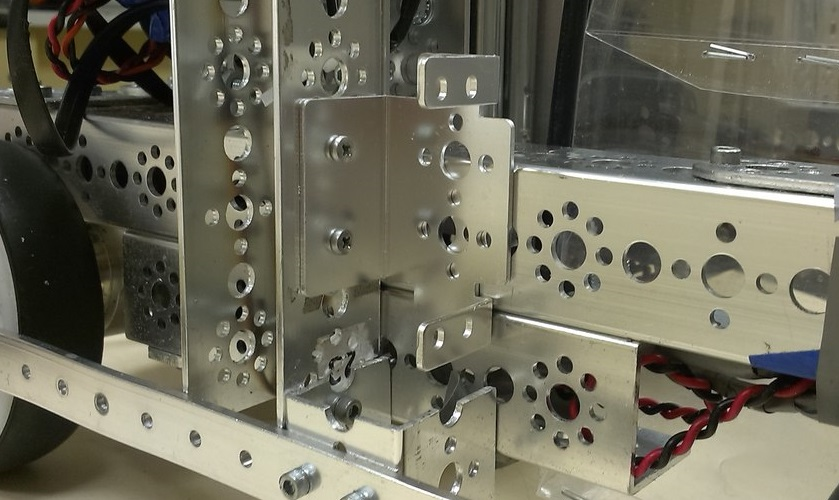
\includegraphics[scale=0.22]{days/23.01.15/images/02}}
	  		\caption{Крепление для сервопривода}
	  	  \end{minipage}
	    \end{figure}

	\end{enumerate}
	
	\item Итоги собрания:
	\begin{enumerate}
		
		\item Механизм захвата мячей доработан, теперь мячи не стопорят его.
		
		\item Крепление для сервопривода установлено, сам сервопривод не установлен.
		
        \item Дополнительный крючок для забрасывания автономных мячей в корзину 30 см не реализован.
		
	\end{enumerate}
	
	\item Задачи для последующих собраний:
	\begin{enumerate}
		
		\item Реализовать дополнительный крючок для автономных мячей и дополнительный захват для корзины.
		
		\item Продолжить тренироваться и сократить время сбора одной порции мячей (5 штук) до минимума.
			
	\end{enumerate}
\end{enumerate}
\fillpage
